%!TEX program = xelatex
\documentclass[11pt]{beamer}

\usepackage{amsmath}
\usepackage{blindtext}
\usepackage{enumitem}

\usetheme{SaoPaulo}  

\title{Python Basics!}
\subtitle{operators, expressions, computing}
\author{CS101 Lecture \#2}
\date{2016-09-28}

\setcounter{showSlideNumbers}{1}

\begin{document}
  \setcounter{showProgressBar}{0}
  \setcounter{showSlideNumbers}{0}

%%%%%%%%%%%%%%%%%%%%%%%%%%%%%%%%%%%%%%%%%%%%%%%%%%%%%%%%%%%%%%%%%%%%%%%%%%%%%%%%
\frame{\titlepage}

%%%%%%%%%%%%%%%%%%%%%%%%%%%%%%%%%%%%%%%%%%%%%%%%%%%%%%%%%%%%%%%%%%%%%%%%%%%%%%%%
\setcounter{framenumber}{0}
\setcounter{showProgressBar}{1}
\setcounter{showSlideNumbers}{1}

%%%%%%%%%%%%%%%%%%%%%%%%%%%%%%%%%%%%%%%%%%%%%%%%%%%%%%%%%%%%%%%%%%%%%%%%%%%%%%%%
\section{Administrivia}

%%%%%%%%%%%%%%%%%%%%%%%%%%%%%%%%%%%%%%%%%%%%%%%%%%%%%%%%%%%%%%%%%%%%%%%%%%%%%%%%
\begin{frame}
  \frametitle{Administrivia}
  \Enlarge
  \begin{itemize}
%  \myitem  Register your i>clickers on the course Compass page.
  %\myitem  
  \item Complete homework before THIS Friday at 6:00 p.m.
  \end{itemize}
\end{frame}

%%%%%%%%%%%%%%%%%%%%%%%%%%%%%%%%%%%%%%%%%%%%%%%%%%%%%%%%%%%%%%%%%%%%%%%%%%%%%%%%
\section{Warmup Quiz}

%%%%%%%%%%%%%%%%%%%%%%%%%%%%%%%%%%%%%%%%%%%%%%%%%%%%%%%%%%%%%%%%%%%%%%%%%%%%%%%%
\begin{frame}
  \frametitle{Question \#1}
  \Enlarge

  A set of instructions executed by a computer to achieve a goal is called:
  \begin{enumerate}[label=\Alph*]
  \item  a process
  \item  a program
  \item  a procedure
  \item  an algorithm
  \end{enumerate}
\end{frame}

%%%%%%%%%%%%%%%%%%%%%%%%%%%%%%%%%%%%%%%%%%%%%%%%%%%%%%%%%%%%%%%%%%%%%%%%%%%%%%%%
\begin{frame}
  \frametitle{Question \#2}
  \Enlarge

  A group of eight bits is called:
  \begin{enumerate}[label=\Alph*]
  \item  a nybble
  \item  a chomp
  \item  a byte
  \item  a gobble
  \end{enumerate}
\end{frame}

%%%%%%%%%%%%%%%%%%%%%%%%%%%%%%%%%%%%%%%%%%%%%%%%%%%%%%%%%%%%%%%%%%%%%%%%%%%%%%%%
\begin{frame}
  \frametitle{Question \#3}
  \Enlarge

  Python is:
  \begin{enumerate}[label=\Alph*]
  \item  a high-level language
  \item  a low-level language
  \end{enumerate}
\end{frame}

%%%%%%%%%%%%%%%%%%%%%%%%%%%%%%%%%%%%%%%%%%%%%%%%%%%%%%%%%%%%%%%%%%%%%%%%%%%%%%%%
\begin{frame}
  \frametitle{Question \#4}
  \Enlarge

  Python is:
  \begin{enumerate}[label=\Alph*]
  \item  an interpreted language
  \item  a compiled language
  \end{enumerate}
\end{frame}

%%%%%%%%%%%%%%%%%%%%%%%%%%%%%%%%%%%%%%%%%%%%%%%%%%%%%%%%%%%%%%%%%%%%%%%%%%%%%%%%
\section{Elements of Programming}

%%%%%%%%%%%%%%%%%%%%%%%%%%%%%%%%%%%%%%%%%%%%%%%%%%%%%%%%%%%%%%%%%%%%%%%%%%%%%%%%
\begin{frame}
  \frametitle{What is a \textbf{literal}?}
  \Enlarge

  \begin{itemize}
  \myitem  Fixed value (noun)
  \myitem  Represents data that doesn't change \\ (\texttt{3} or \texttt{'firefly'})
  \end{itemize}
\end{frame}

%%%%%%%%%%%%%%%%%%%%%%%%%%%%%%%%%%%%%%%%%%%%%%%%%%%%%%%%%%%%%%%%%%%%%%%%%%%%%%%%
\begin{frame}
  \frametitle{Executing a literal?}
  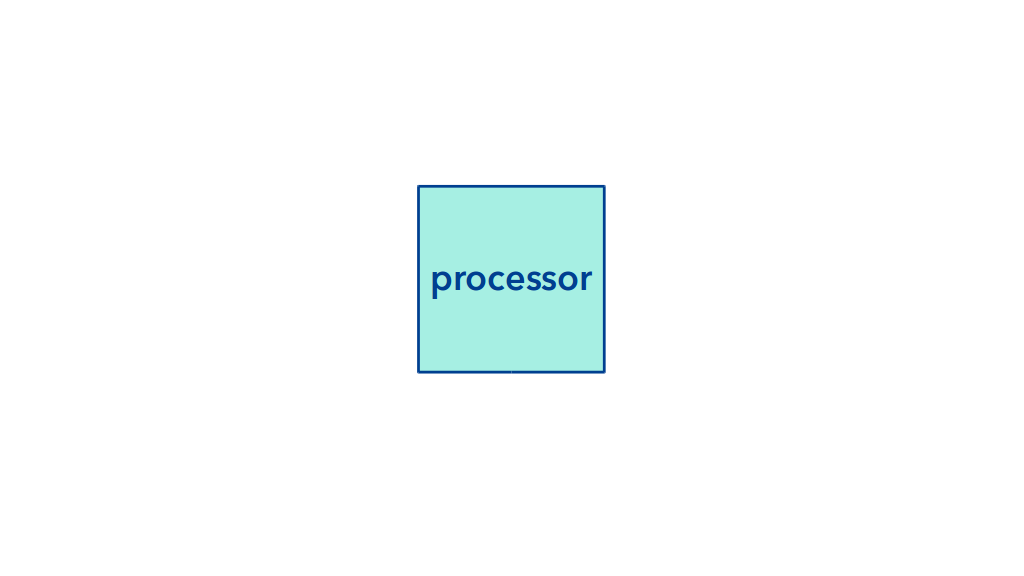
\includegraphics[width=\textwidth]{./img/computer.png}
\end{frame}

%%%%%%%%%%%%%%%%%%%%%%%%%%%%%%%%%%%%%%%%%%%%%%%%%%%%%%%%%%%%%%%%%%%%%%%%%%%%%%%%
\begin{frame}
  \frametitle{Executing a literal?}
  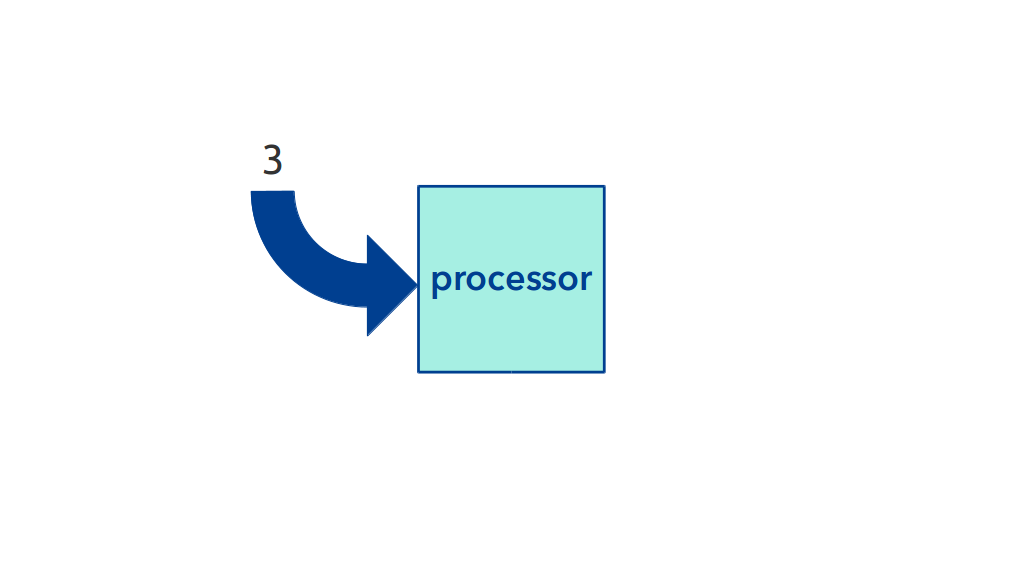
\includegraphics[width=\textwidth]{./img/computer-literal-0.png}
\end{frame}

%%%%%%%%%%%%%%%%%%%%%%%%%%%%%%%%%%%%%%%%%%%%%%%%%%%%%%%%%%%%%%%%%%%%%%%%%%%%%%%%
\begin{frame}
  \frametitle{Executing a literal?}
  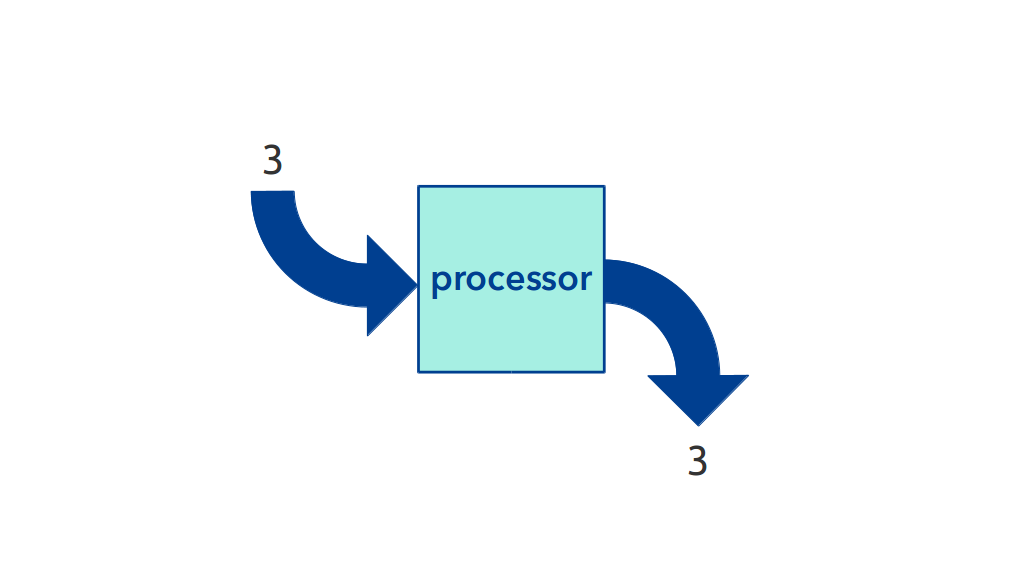
\includegraphics[width=\textwidth]{./img/computer-literal-1.png}
\end{frame}

%%%%%%%%%%%%%%%%%%%%%%%%%%%%%%%%%%%%%%%%%%%%%%%%%%%%%%%%%%%%%%%%%%%%%%%%%%%%%%%%
\begin{frame}
  \frametitle{What is an \textbf{operator}?}
  \Enlarge

  \begin{itemize}
  \myitem  Manipulates data (verb)
  \end{itemize}
\end{frame}

%%%%%%%%%%%%%%%%%%%%%%%%%%%%%%%%%%%%%%%%%%%%%%%%%%%%%%%%%%%%%%%%%%%%%%%%%%%%%%%%
\begin{frame}
  \frametitle{Executing an operator?}
  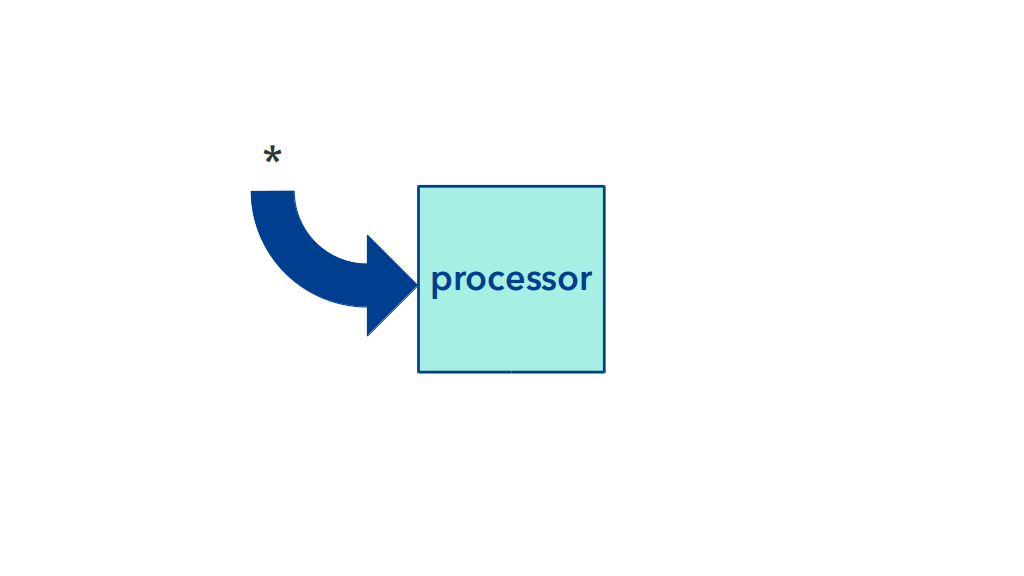
\includegraphics[width=\textwidth]{./img/computer-operator-0.png}
\end{frame}

%%%%%%%%%%%%%%%%%%%%%%%%%%%%%%%%%%%%%%%%%%%%%%%%%%%%%%%%%%%%%%%%%%%%%%%%%%%%%%%%
\begin{frame}
  \frametitle{It needs a statement to make sense!}
  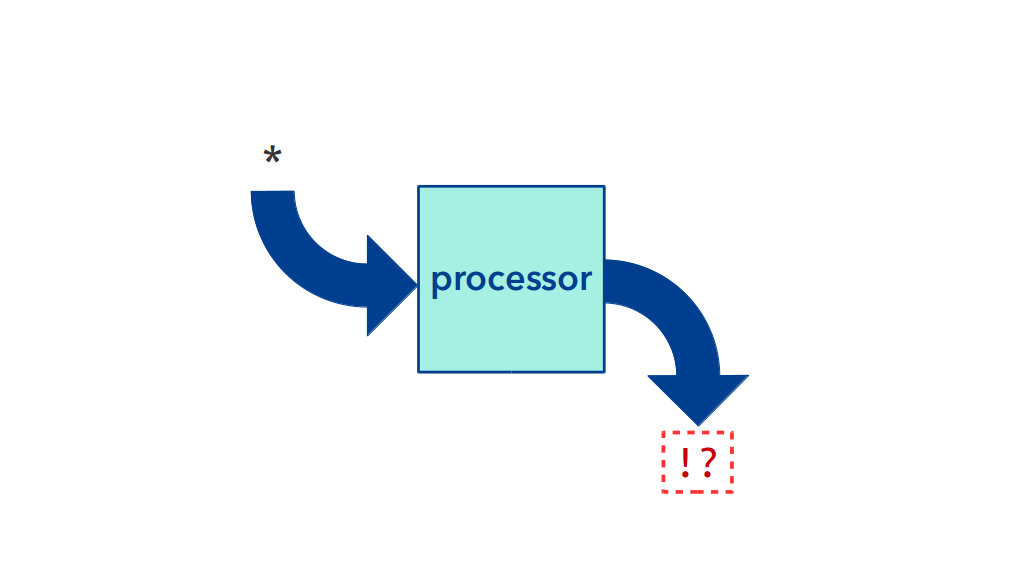
\includegraphics[width=\textwidth]{./img/computer-operator-1.png}
\end{frame}

%%%%%%%%%%%%%%%%%%%%%%%%%%%%%%%%%%%%%%%%%%%%%%%%%%%%%%%%%%%%%%%%%%%%%%%%%%%%%%%%
\begin{frame}
  \frametitle{What is an \textbf{expression}?}
  \Enlarge

  \begin{itemize}
  \myitem  Combines literals and operators (phrase) \pause
  \myitem  Produce a new value
    \begin{itemize}
    \mysubitem  \texttt{3 * 5}
    \mysubitem  \texttt{100 - 23}
    \end{itemize}
  \end{itemize}
\end{frame}

%%%%%%%%%%%%%%%%%%%%%%%%%%%%%%%%%%%%%%%%%%%%%%%%%%%%%%%%%%%%%%%%%%%%%%%%%%%%%%%%
\begin{frame}
  \frametitle{Executing an expression?}
  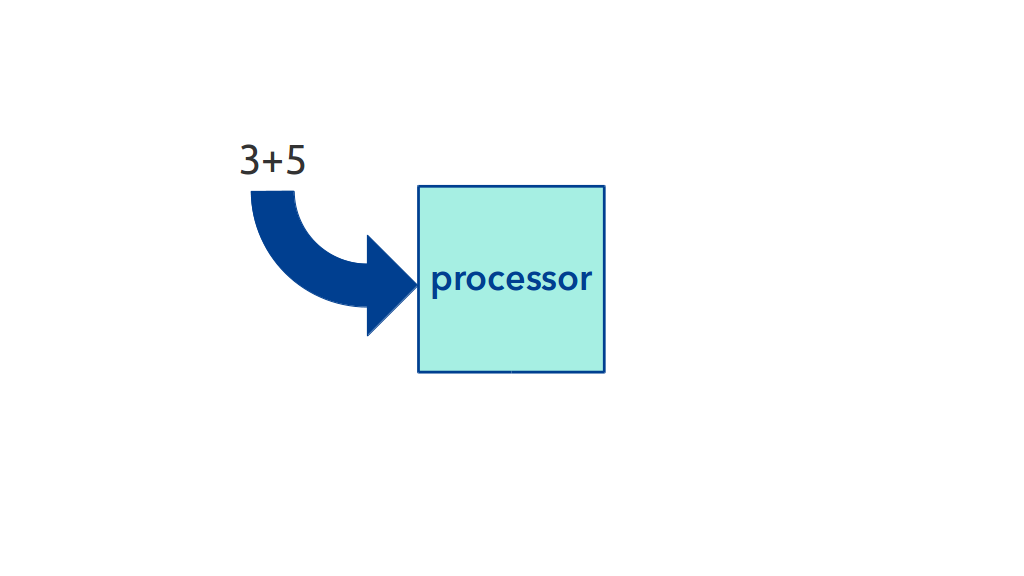
\includegraphics[width=\textwidth]{./img/computer-expression-0.png}
\end{frame}

%%%%%%%%%%%%%%%%%%%%%%%%%%%%%%%%%%%%%%%%%%%%%%%%%%%%%%%%%%%%%%%%%%%%%%%%%%%%%%%%
\begin{frame}
  \frametitle{Executing an expression?}
  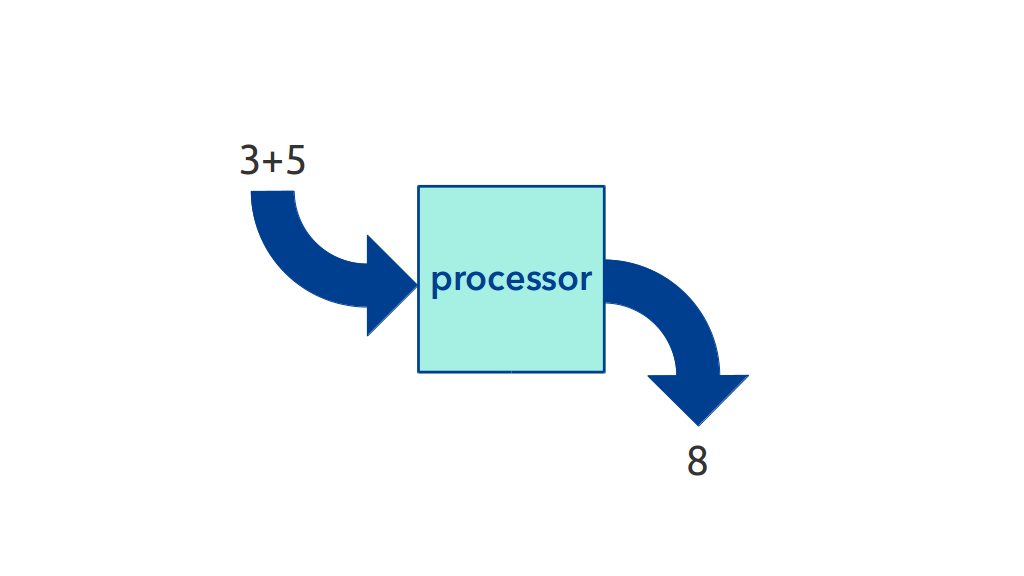
\includegraphics[width=\textwidth]{./img/computer-expression-1.png}
\end{frame}

%%%%%%%%%%%%%%%%%%%%%%%%%%%%%%%%%%%%%%%%%%%%%%%%%%%%%%%%%%%%%%%%%%%%%%%%%%%%%%%%
\begin{frame}
  \frametitle{What is an \textbf{expression}?}
  \Enlarge

  \begin{itemize}
  \myitem  Can be arbitrarily complicated
    \begin{itemize}
    \mysubitem  \texttt{3 + 8*5 + 4 - 7/100}
    \end{itemize}
  \end{itemize}
\end{frame}

%%%%%%%%%%%%%%%%%%%%%%%%%%%%%%%%%%%%%%%%%%%%%%%%%%%%%%%%%%%%%%%%%%%%%%%%%%%%%%%%
\begin{frame}
  \frametitle{Question}
  \Enlarge

  $\mathtt{1 + 1 * 2} \overset{?}{=}$
  \begin{enumerate}[label=\Alph*]
  \item  4
  \item  3
  \item  Something else
  \end{enumerate}
\end{frame}

%%%%%%%%%%%%%%%%%%%%%%%%%%%%%%%%%%%%%%%%%%%%%%%%%%%%%%%%%%%%%%%%%%%%%%%%%%%%%%%%
\begin{frame}
  \frametitle{Question}
  \Enlarge

  $\mathtt{23 + 6 / 2 - 4} \overset{?}{=}$
  \begin{enumerate}[label=\Alph*]
  \item  22
  \item  18
  \item  -9
  \item  Something else
  \end{enumerate}
\end{frame}

%%%%%%%%%%%%%%%%%%%%%%%%%%%%%%%%%%%%%%%%%%%%%%%%%%%%%%%%%%%%%%%%%%%%%%%%%%%%%%%%
\begin{frame}
  \frametitle{Use parentheses!}
  \Enlarge

  $\mathtt{23 + \left(6 / 2\right) - 4}$ is always clearer.
\end{frame}

%%%%%%%%%%%%%%%%%%%%%%%%%%%%%%%%%%%%%%%%%%%%%%%%%%%%%%%%%%%%%%%%%%%%%%%%%%%%%%%%
\begin{frame}
  \frametitle{What are some other operators?}
  \Enlarge

  \begin{itemize}
  \myitem  exponentiation, \texttt{**} \pause
  \myitem  modulus, \texttt{\%}  (important) \pause
  \myitem  floor division, \texttt{//}
  \end{itemize}
\end{frame}

%%%%%%%%%%%%%%%%%%%%%%%%%%%%%%%%%%%%%%%%%%%%%%%%%%%%%%%%%%%%%%%%%%%%%%%%%%%%%%%%
\begin{frame}
  \frametitle{What are some other operators?}
  \Enlarge

  \begin{itemize}
  \myitem  bitwise \texttt{OR}, \texttt{|}
  \myitem  bitwise \texttt{XOR}, \texttt{\^{}}
  \myitem  bitwise \texttt{AND}, \texttt{\&}
  \myitem  bitwise left shift, \texttt{<{}<}
  \myitem  bitwise right shift, \texttt{>{}>}
  \end{itemize}
\end{frame}

%%%%%%%%%%%%%%%%%%%%%%%%%%%%%%%%%%%%%%%%%%%%%%%%%%%%%%%%%%%%%%%%%%%%%%%%%%%%%%%%
\begin{frame}
  \frametitle{Example}
  \Enlarge

  \texttt{1 \^{} 2} $\overset{?}{=}$
  \\
  \begin{enumerate}[label=\Alph*]
  \item  0
  \item  1
  \item  2
  \item  3
  \end{enumerate}
\end{frame}

%TODO: make a graphic
%http://www.tutorialspoint.com/python/bitwise_operators_example.htm

%%%%%%%%%%%%%%%%%%%%%%%%%%%%%%%%%%%%%%%%%%%%%%%%%%%%%%%%%%%%%%%%%%%%%%%%%%%%%%%%
\begin{frame}
  \frametitle{So what?}
  \Enlarge

  \begin{itemize}
  \myitem  The machine state hasn't changed. \pause
  \myitem  Programs are complex, and we need to remember results.
  \end{itemize}
\end{frame}

%%%%%%%%%%%%%%%%%%%%%%%%%%%%%%%%%%%%%%%%%%%%%%%%%%%%%%%%%%%%%%%%%%%%%%%%%%%%%%%%
\begin{frame}
  \frametitle{How do we keep values around?}
  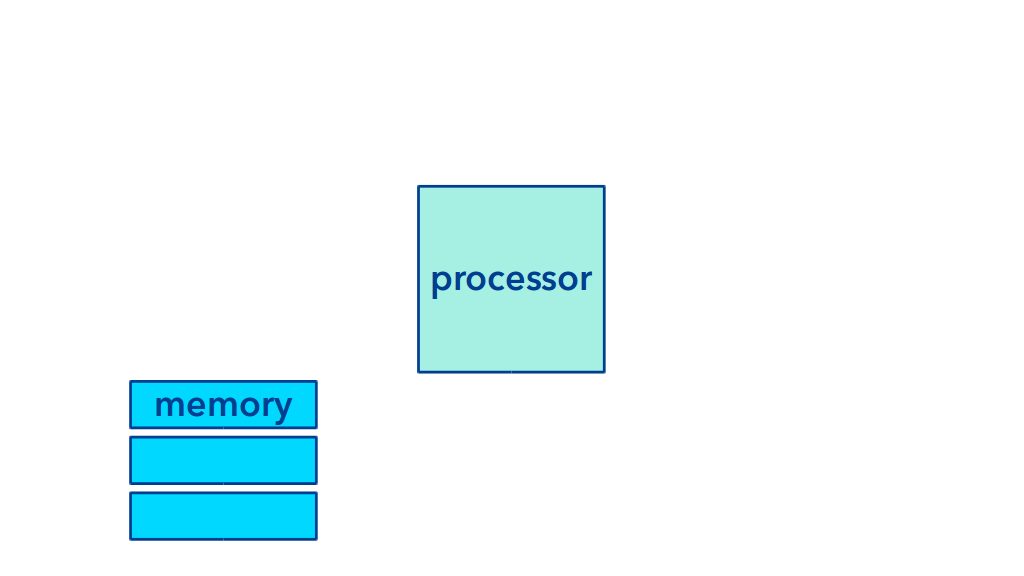
\includegraphics[width=\textwidth]{./img/computer-memory.png}
\end{frame}

%%%%%%%%%%%%%%%%%%%%%%%%%%%%%%%%%%%%%%%%%%%%%%%%%%%%%%%%%%%%%%%%%%%%%%%%%%%%%%%%
\begin{frame}
  \frametitle{How do we keep values around?}
  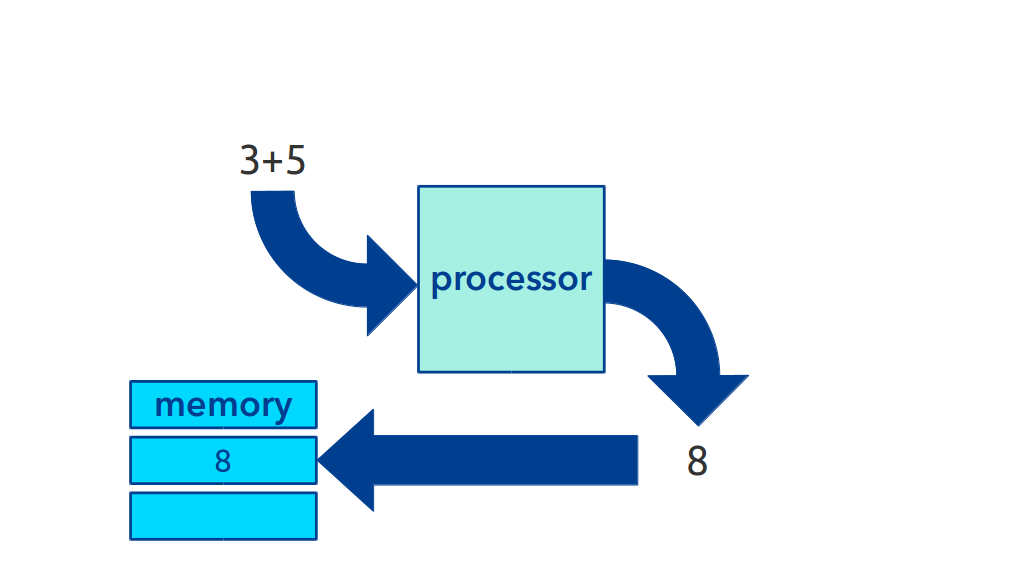
\includegraphics[width=\textwidth]{./img/computer-memory-0.png}
\end{frame}

%%%%%%%%%%%%%%%%%%%%%%%%%%%%%%%%%%%%%%%%%%%%%%%%%%%%%%%%%%%%%%%%%%%%%%%%%%%%%%%%
\begin{frame}
  \frametitle{How do we reuse values?}
  \Enlarge

  \begin{itemize}
  \myitem  Low-level languages refer directly to memory address:
  \begin{tabular}{*{27}{l}}
    \texttt{ADD DATA AT}     & \texttt{10101101 11010100} \\
    \texttt{TO DATA AT}      & \texttt{11010100 01001001} \\
    \texttt{STORE RESULT AT} & \texttt{00001101 01001110} \\
  \end{tabular}
  \end{itemize}
\end{frame}

%%%%%%%%%%%%%%%%%%%%%%%%%%%%%%%%%%%%%%%%%%%%%%%%%%%%%%%%%%%%%%%%%%%%%%%%%%%%%%%%
\begin{frame}
  \frametitle{What is a \textbf{variable}?}
  \Enlarge

  \begin{itemize}
  \myitem  The solution:  \textcolor{CS101GradBot}{name memory locations!} \pause
  \myitem  Variables name a memory location \pause
  \myitem  Variables store a value \pause
  \myitem  This value can change over time---it is a placeholder.
  \end{itemize}
\end{frame}

%%%%%%%%%%%%%%%%%%%%%%%%%%%%%%%%%%%%%%%%%%%%%%%%%%%%%%%%%%%%%%%%%%%%%%%%%%%%%%%%
\begin{frame}
  \frametitle{What new operator do we need?}
  \Enlarge

  \begin{itemize}
  \myitem  assignment, \texttt{=} (single equals sign)
  \end{itemize}
\end{frame}

%%%%%%%%%%%%%%%%%%%%%%%%%%%%%%%%%%%%%%%%%%%%%%%%%%%%%%%%%%%%%%%%%%%%%%%%%%%%%%%%
\begin{frame}
  \frametitle{How do we reuse values?}
  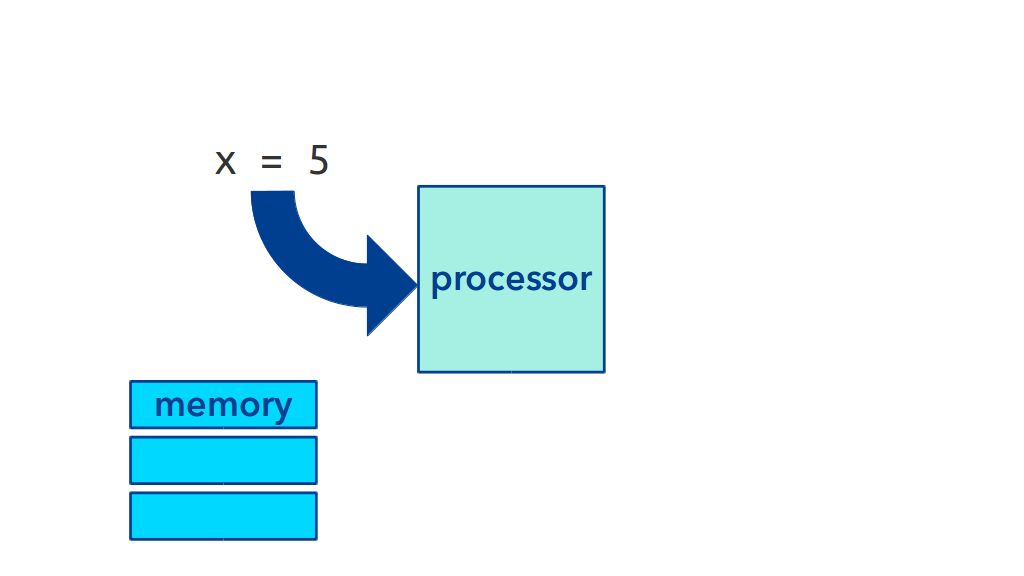
\includegraphics[width=\textwidth]{./img/computer-memory-1.png}
\end{frame}

%%%%%%%%%%%%%%%%%%%%%%%%%%%%%%%%%%%%%%%%%%%%%%%%%%%%%%%%%%%%%%%%%%%%%%%%%%%%%%%%
\begin{frame}
  \frametitle{How do we reuse values?}
  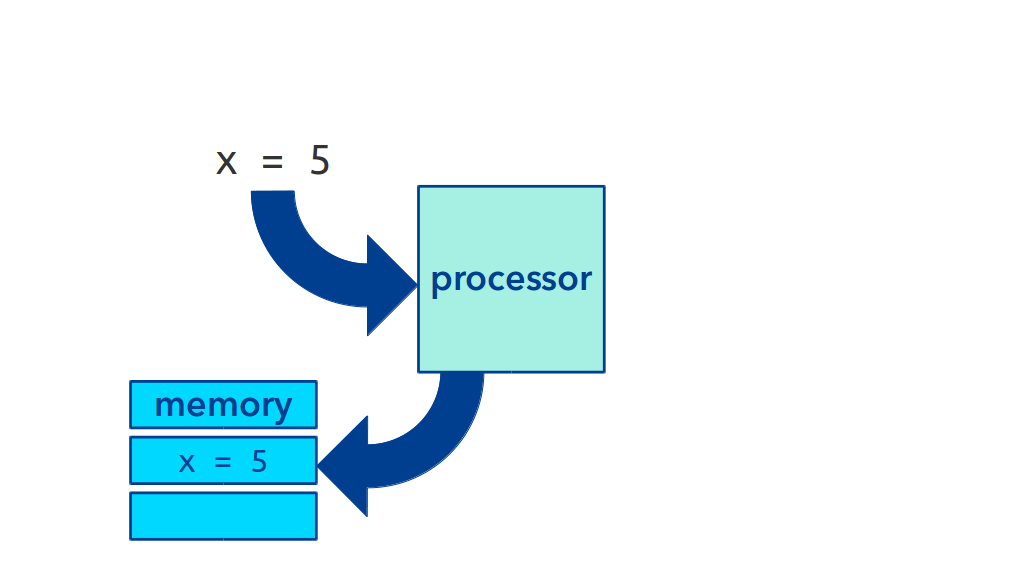
\includegraphics[width=\textwidth]{./img/computer-memory-2.png}
\end{frame}

%%%%%%%%%%%%%%%%%%%%%%%%%%%%%%%%%%%%%%%%%%%%%%%%%%%%%%%%%%%%%%%%%%%%%%%%%%%%%%%%
\begin{frame}
  \frametitle{How do we reuse values?}
  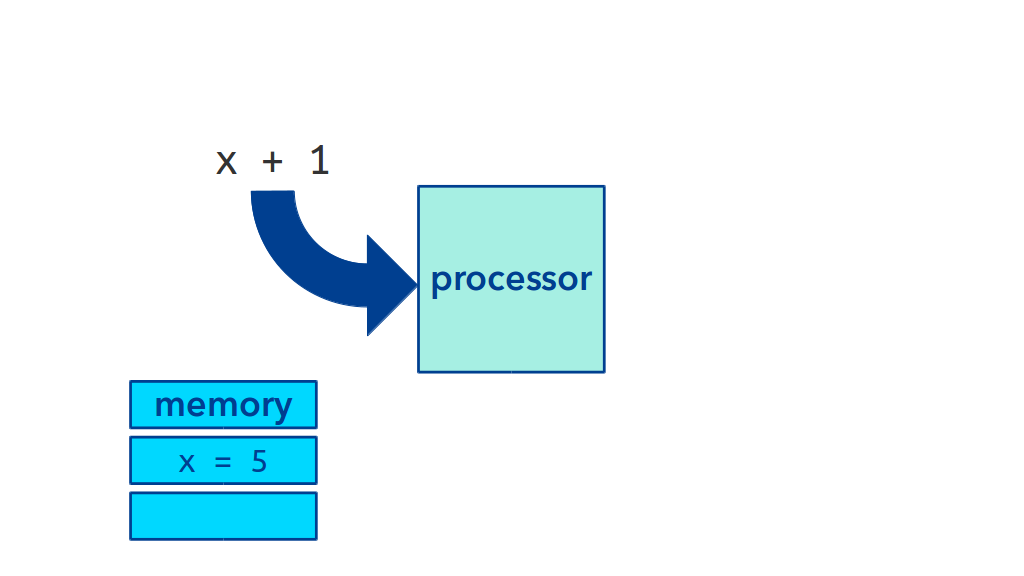
\includegraphics[width=\textwidth]{./img/computer-memory-3.png}
\end{frame}

%%%%%%%%%%%%%%%%%%%%%%%%%%%%%%%%%%%%%%%%%%%%%%%%%%%%%%%%%%%%%%%%%%%%%%%%%%%%%%%%
\begin{frame}
  \frametitle{How do we reuse values?}
  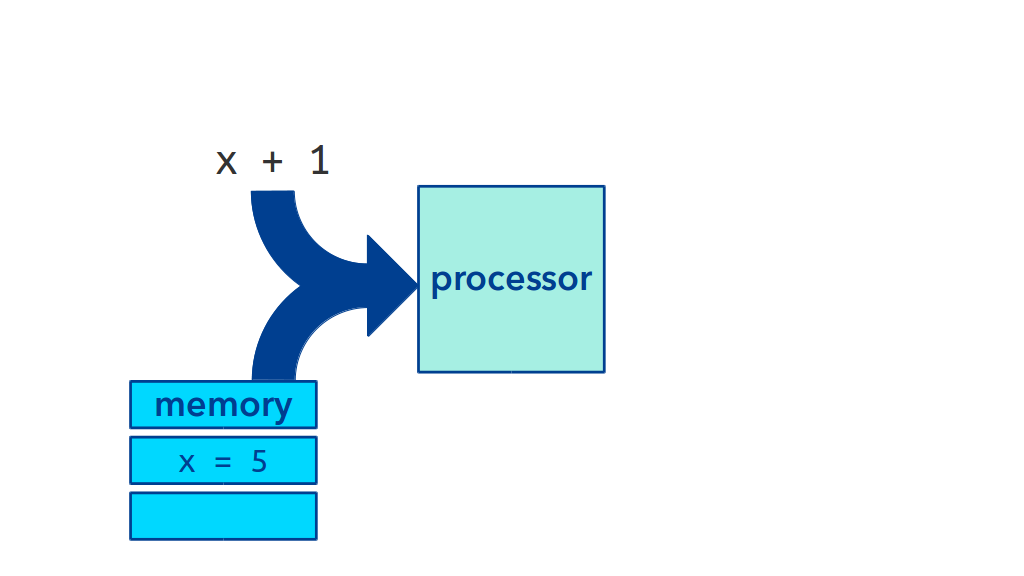
\includegraphics[width=\textwidth]{./img/computer-memory-4.png}
\end{frame}

%%%%%%%%%%%%%%%%%%%%%%%%%%%%%%%%%%%%%%%%%%%%%%%%%%%%%%%%%%%%%%%%%%%%%%%%%%%%%%%%
\begin{frame}
  \frametitle{How do we reuse values?}
  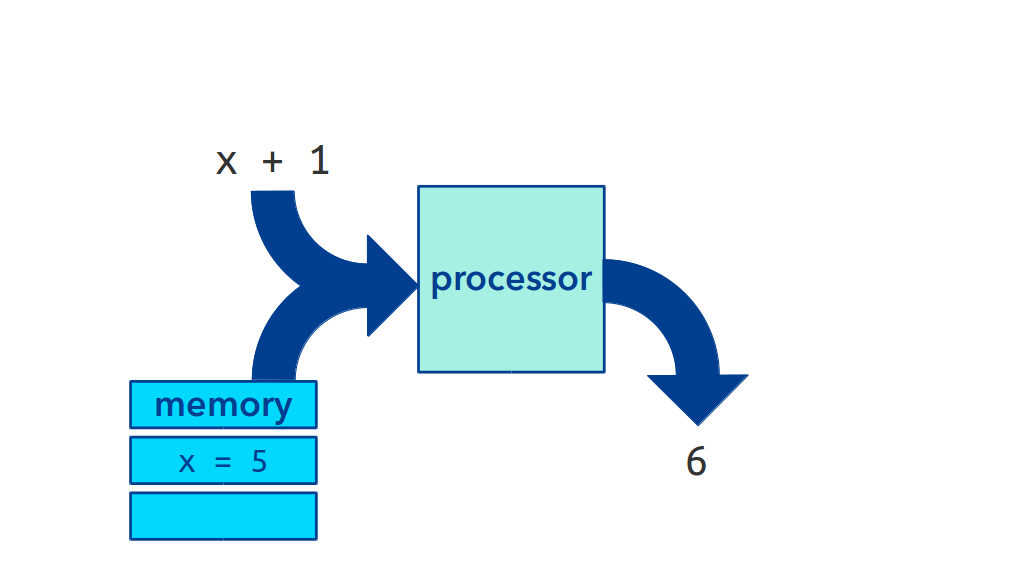
\includegraphics[width=\textwidth]{./img/computer-memory-5.png}
\end{frame}

%%%%%%%%%%%%%%%%%%%%%%%%%%%%%%%%%%%%%%%%%%%%%%%%%%%%%%%%%%%%%%%%%%%%%%%%%%%%%%%%
\begin{frame}
  \frametitle{Example}
  \Enlarge

  What value is stored in the variable \texttt{x}? \\
  \texttt{x = 17 + 7*9}
  \begin{enumerate}[label=\Alph*]
  \item  3
  \item  31
  \item  55
  \item  78
  \end{enumerate}
\end{frame}

%%%%%%%%%%%%%%%%%%%%%%%%%%%%%%%%%%%%%%%%%%%%%%%%%%%%%%%%%%%%%%%%%%%%%%%%%%%%%%%%
\begin{frame}
  \frametitle{Example}
  \Enlarge

  What value is stored in the variable \texttt{x}? \\
  \texttt{x = 17 + 7*9} \\
  \texttt{x = 3}
  \begin{enumerate}[label=\Alph*]
  \item  0
  \item  1
  \item  2
  \item  3
  \end{enumerate}
\end{frame}

%%%%%%%%%%%%%%%%%%%%%%%%%%%%%%%%%%%%%%%%%%%%%%%%%%%%%%%%%%%%%%%%%%%%%%%%%%%%%%%%
\begin{frame}
  \frametitle{What is a \textbf{statement}?}
  \Enlarge

  \begin{itemize}
  \myitem  A statement changes the state of the computer (sentence) \pause
  \myitem  Example:  an assignment
  \end{itemize}
\end{frame}

%%%%%%%%%%%%%%%%%%%%%%%%%%%%%%%%%%%%%%%%%%%%%%%%%%%%%%%%%%%%%%%%%%%%%%%%%%%%%%%%
\begin{frame}
  \frametitle{What is a \textbf{program}?}
  \Enlarge

  \begin{itemize}
  \myitem  Programs consist of series of statements: \pause
    \begin{itemize}
    \mysubitem  A script is a file containing a series of Python statement. \pause
    \mysubitem  A notebook (as we use in the lab) also collects series of Python statements. \pause
    \mysubitem  These are stored in text (there’s no magic, just text). \pause
  \end{itemize}
  \myitem  Each instruction is executed in order from top to bottom—together, these statements make up a program.
  \end{itemize}
 \end{frame}

%%%%%%%%%%%%%%%%%%%%%%%%%%%%%%%%%%%%%%%%%%%%%%%%%%%%%%%%%%%%%%%%%%%%%%%%%%%%%%%%
\begin{frame}[fragile]
  \frametitle{Our first program}
  \Enlarge

  \begin{semiverbatim}
x = 10
y = x ** 2
y = y + y
  \end{semiverbatim}
\end{frame}

%%%%%%%%%%%%%%%%%%%%%%%%%%%%%%%%%%%%%%%%%%%%%%%%%%%%%%%%%%%%%%%%%%%%%%%%%%%%%%%%
\section{Reminders}

%%%%%%%%%%%%%%%%%%%%%%%%%%%%%%%%%%%%%%%%%%%%%%%%%%%%%%%%%%%%%%%%%%%%%%%%%%%%%%%%
\begin{frame}
  \frametitle{Reminders}
  \Enlarge

  \begin{itemize}
  %\myitem  Register your i>clicker on Compass.
  %\myitem  
  \item Homework \#1 due Friday, Sept.\ 30, 6:00 p.m.
  \end{itemize}
\end{frame}

\end{document}
